\documentclass[10pt]{article}
\usepackage[margin=0.65in]{geometry}
\usepackage{graphicx,booktabs,amsmath,amssymb,hyperref}
\hypersetup{colorlinks=true,urlcolor=blue}
\setlength{\parindent}{0pt}\setlength{\parskip}{5pt}
\begin{document}
{\Large\bfseries Full original quadratic row-space audit}\par
\textbf{Native PCC-20261117-f9b20c. Producer unsigned/unverified.}\par
Constant combinations of the original unassigned equations add no input-only
polynomial for either explicit keep set. Independent, formal or signed
checking remains pending.
\begin{center}\begin{tabular}{lrrrr}
\toprule Projection &Kept&Input rank&Auxiliary rank&New dimension\\\midrule
Raw parameter pairs&12&6&1083/1083&0\\
All named inputs&204&198&891/891&0\\\bottomrule
\end{tabular}\end{center}
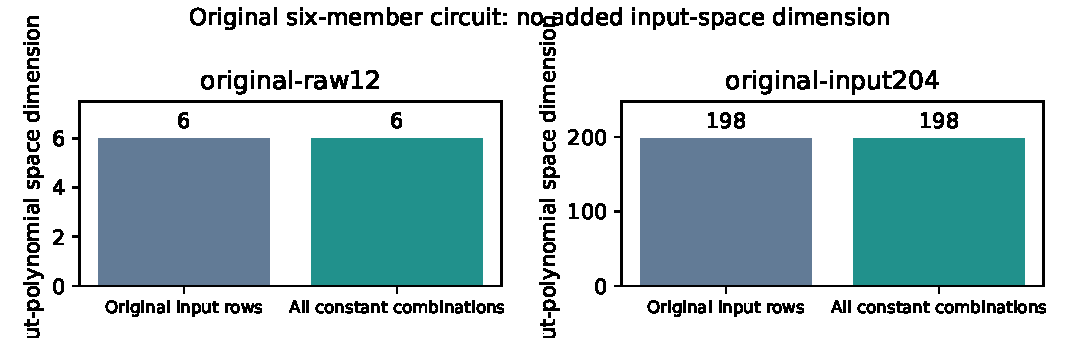
\includegraphics[width=\linewidth]{ranks.pdf}
\textbf{Original input.} All 1059 variables,1089 equations and3323 terms of
the frozen original $q=213156431$, arity-six circuit over $p=2^{255}-19$
remain. No witness is read, equation or guard removed, or root solver called.
A fixed target is not a growing-family statement.

\textbf{Complete row-space argument.} Split equations into input-only $U$
and remaining $R$. Project $R$ onto auxiliary monomials, obtaining $A$.
For constant field weights, exactly
\[
\operatorname{span}(U,R)\cap F[\text{inputs}]_{\leq2}
=\operatorname{span}(U)+\{cR:cA=0\}.
\]
Each transformed row is directly reconstructed from original rows, with a
nonzero lower-triangular origin diagonal. Fresh unit pivots have every earlier
pivot zero. Hence zero rows give the complete left kernel. Both projections
have zero kernel; separately checked input ranks stay 6 and198. This is
classical linear algebra, not a new algorithm or compiler/group/primality proof.

\textbf{Controls.} Seven fixed static cases complete: five hand-derived
$F_{29}$ matrices and two original projections. The matrices cover a new
quadratic relation,private-pivot null,existing input,zero image,and constant
conflict. Eight mutations,extra serialization fields and oversized input
refuse; three forced quotas refuse in generator and reader. First release
unit,strict all-target Clippy and build pass. First fmt refusal and preformat
source remain. All native source is unchanged after qualification.
\newpage
{\large\bfseries Exact boundary, custody and next check}\par
\includegraphics[width=\linewidth]{pipeline.pdf}
\textbf{V3 closure.} This producer finite certificate concerns only the
exact unassigned constant row-space claim and keep sets,subject to independent
checking. It is stronger than a bounded-slice null. It is not an ideal,
solving-degree,all-target or index-calculus exclusion.

Ordinary unit substitution already escapes this space: $x=1,xy=2$ imply
$y=2$ through the polynomial multiple $y(x-1)$. Existing conditional engines
already specialize equations; their proposed univariate extractor remains
open. A quadratic root extractor alone cannot create a missing row polynomial.

\textbf{Next proposed check.} Audit the degree-two module after exact affine
quotient or controlled variable multiples of linear equations. Review old
affine-closure code and retained reservation failures first. Preserve all
original equations and charge substitution fill,storage and complete added
work. Freeze a distinct protocol before calls. No successor is running or
scheduled. Higher-degree multiples and symbolic target-independent rank are
separate hypotheses. Useful yield,full cold cost,family scaling,selection,
rank,kernel and recovery obligations remain open.

\textbf{Admission, not performance.} At most4096 variables,8192 rows,
32768 terms and degree two. Each generator/reader separately admits50 million
charged events,eight million coefficient writes and one million represented
certificate entries. These are static quotas,not normalized field work,
allocator/peak RSS bounds,timing or complete attack cost. Original solver caps
remain unchanged. No paid run,sampling,benchmark or full-base enumeration.
The figure copies recorded dimensions; canonical performance/exponent graphs
and benchmarks stay unchanged.

\textbf{Frozen custody.} Seven source/input files,including unchanged old
gzip,are archived in32272 bytes (SHA-256 prefix\texttt{2f62273d}). Whole native
round:23 files,3137597 bytes,compressed losslessly to54716 bytes
(\texttt{2c9c3816}). The5554-byte Rust aggregate is also at its real path.
Copied executable\texttt{467c0e23},all seven compiled bindings and separately
copied qualifier match. Build,pre-call and post-call records are distinct.
No source edits or native reruns for report/publication metadata.

\textbf{Primary context.} Courtois,Klimov,Patarin,Shamir,
\emph{Efficient Algorithms for Solving Overdefined Systems of Multivariate
Polynomial Equations},Definition3.01 steps2--3:
\url{https://www.nicolascourtois.com/papers/xlfull.pdf}.
No generic-rank heuristic is imported. KB unavailable; inaccessible Diem full
text not used. Original criteria/source/report bindings remain unchanged.

\textbf{Reproduction.} Study\texttt{rowspace-audit-v1/REPRODUCE.md}; isolated
Rust crate\texttt{tools/torus-rowspace-audit}. Public systems,keep lists,
complete certificates,summaries and first attempts remain. The direct native
reader is producer code and confers no signed PCC standing.
\end{document}
